% STEEL-in-Rust validation letter -- draft
%
% Requires mnras.cls and mnras.bst (Royal Astronomical Society /
% Oxford University Press house style), not included here. Download
% from https://academic.oup.com/mnras/pages/General_Instructions
% and place alongside this file before compiling.
%
% This is a first draft assembled from the port-validation work in
% docs/RESULTS_REPRODUCTION.md, docs/PORT_CORRECTIONS.md, and
% docs/VALIDATION.md. Numbers and figures are real (regenerated by the
% scripts in Scripts/Validation/); the prose needs an author pass.

\documentclass[fleqn,usenatbib]{mnras}

\usepackage{graphicx}
\usepackage{amsmath}
\usepackage{amssymb}
\usepackage{xcolor}

\title[STEEL in Rust]{A dependency-injection port of the STEEL statistical semi-empirical model to Rust, and a three-way validation against the published results}

\author[Grylls et al.]{
Philip J. Grylls$^{1}$\thanks{E-mail: p.grylls@soton.ac.uk}
\\
$^{1}$Department for Physics and Astronomy, University of Southampton, Highfield SO17 1BJ, UK
}

\pubyear{2026}

\begin{document}
\label{firstpage}
\pagerange{\pageref{firstpage}--\pageref{lastpage}}
\maketitle

\begin{abstract}
STEEL (Statistical sEmi-Empirical modeL) is the dark-matter-accretion-history-based
semi-empirical galaxy formation model behind three papers
\citep{Grylls2019a,Grylls2020,Grylls2020b}. The original code is a mix of
Python and hand-tuned Cython that no longer runs on a current software
stack: it depends on removed \textsc{numpy}/\textsc{scipy}/\textsc{pandas}
APIs, a machine-specific compiled Fortran binary for the halo mass
accretion history, and an interactive confirmation prompt that blocks
unattended execution. We describe a from-scratch, dependency-injected
Rust reimplementation (\texttt{rs-steel}) built around one trait per
physical process -- cosmology, halo growth, halo and subhalo mass
functions, merger time-scale, stellar--halo mass relation, star
formation, quenching, and stellar stripping -- and validate it against
both the original code and a corrected version of it (\texttt{py-corrected}) on
every headline results figure across all three papers. In deterministic
mode (scatter disabled on both sides) every integrated quantity we
compare agrees to better than 0.5\% between \texttt{py-corrected} and
\texttt{rs-steel}, with disagreement concentrated in the sparse
high-mass tail where individual bins hold at most one object. The
reimplementation runs $4.5\times$ faster than the (already
Cython-accelerated) Python on the published parameter grid. In the
process of building and validating this reproduction we found and fixed
a number of defects in the code branch the three papers were run from,
none individually dramatic but collectively shifting the shape (not the
normalisation) of the merger accretion history and pair-fraction outputs
by tens of per cent under the corrections' combined effect. We give the
full list, quantify which published results move and by how much, and
argue that a from-scratch, independently-typed reimplementation
validated this way is a practical and under-used check on
semi-empirical model code.
\end{abstract}

\begin{keywords}
methods: numerical -- methods: statistical -- galaxies: haloes -- galaxies: statistics
\end{keywords}

\section{Introduction}
\label{sec:intro}

Semi-empirical models connect dark matter haloes to galaxies through
observationally calibrated relations (typically abundance matching)
rather than the coupled hydrodynamics and sub-grid physics of a
cosmological simulation, or the merger-tree bookkeeping of a
semi-analytic model. STEEL \citep{Grylls2019a} took this a step further,
replacing discrete dark matter merger trees with a \emph{statistical}
accretion history: at every redshift step, the halo mass function and an
analytic mass-accretion-history model together give the expected number
density and mass of subhaloes accreted onto a halo of any given mass, with
no dependence on simulation volume or resolution. \citet{Grylls2020}
extended this to derive star formation histories self-consistently from
the growth of the dark matter and the abundance-matched stellar mass, and
\citet{Grylls2020b} used the same machinery to study how the choice of
stellar mass estimator propagates into the inferred galaxy pair fraction.

Software written for one project rarely survives contact with a second
one unmodified, and STEEL is no exception. Re-running the published code
seven years on surfaces three separate problems. First, \emph{it does not
run}: the code imports \textsc{pandas}, \textsc{numpy} and \textsc{scipy}
APIs removed in the intervening major versions (\S\ref{sec:repro}), and the
halo mass accretion history is computed by shelling out to a Fortran
binary compiled with a machine-specific output path. Second, where it
does run, several code paths silently compute something other than what
the papers describe -- not edge cases, but the exact configurations the
published figures use (\S\ref{sec:bugs}). Third, there is no independent
implementation to check any of this against: a bug shared between the
code and the papers built from it is invisible from inside that one
codebase.

We address this by writing a second, independent implementation from the
model description in the three papers, in a different language, with a
different type system and a different numerical stack, and comparing the
two on every result each paper reports. Agreement is evidence the port
(and, to the extent they overlap, the original) is doing what the papers
say; disagreement identifies either a porting error or a defect in the
original that the comparison itself localises. This letter reports that
comparison. \S\ref{sec:repro} documents the reproducibility failure
concretely. \S\ref{sec:port} summarises the Rust implementation.
\S\ref{sec:method} describes the three-way validation methodology.
\S\ref{sec:results} gives the results: numerical fidelity, the defects
found and their impact, wall-clock performance, and a figure-by-figure
reproduction of the three papers' results. \S\ref{sec:discuss} discusses
what generalises.

\section{The original code no longer runs}
\label{sec:repro}

Attempting to execute \texttt{STEEL.py} as published fails at import time:
\texttt{CentralPostprocessing.py} constructs an SDSS-comparison object as
a module-level side effect, so post-processing cannot be imported without
first obtaining the observational catalogue, which is not distributed
with the code. Past that point, \texttt{Scripts/CentralPostprocessing.py}
calls \texttt{pandas.Series.get\_values()} (removed in pandas 1.0),
\texttt{scipy.interpolate.interp2d} and
\texttt{scipy.integrate.cumtrapz} (removed in SciPy 1.14), and reads
whitespace-delimited files with the \texttt{delim\_whitespace} keyword
(removed in pandas 2.2). None of these are exotic APIs; they are
mainstream functions removed by ordinary version churn over seven years.
Separately, \texttt{Functions.py::Halogrowth} obtains the halo mass
accretion history by shelling out to \texttt{getPWGH}, a compiled Fortran
binary invoked with a hardcoded, machine-specific output path -- it has
no standalone Python entry point, so nothing that calls \texttt{Halogrowth}
runs on a machine that is not the original author's. \texttt{STEEL.py}
itself blocks on an interactive confirmation prompt before running,
precluding unattended execution. We built two pinned virtual
environments (one on the last Python/NumPy/SciPy/pandas versions that
still provide the removed APIs, one modern) and patched around each of
these individually to obtain a runnable baseline; that baseline, not the
repository as published, is what we call \texttt{py-as-is} throughout.

\section{Motivation}
\label{sec:mot}

Why revisit a model whose only implementation no longer runs
(\S\ref{sec:repro})? Two things make this a good moment to. The first is
practical: this port was written with substantial large-language-model
assistance, at a fraction of the engineering time a from-scratch
reimplementation would otherwise take. The second is what that lower
cost unlocks. STEEL's stated purpose was never only to reproduce the
three published papers -- it was meant as a testbed for the internal
self-consistency of evolved stellar-mass--halo-mass (SMHM) relations, in
which a new SMHM model, quenching prescription, or stripping law could
be dropped in and checked against the same statistical accretion-history
machinery. What blocked that use case was never the physics but the
integration cost: coding a new prescription and wiring it into the
surrounding pipeline without silently breaking something else was
expensive enough that STEEL produced three papers and stopped, rather
than becoming the general-purpose testbed it was designed to be.

The dependency-injection structure described in \S\ref{sec:port} is
what turns a lower integration cost into a testbed rather than just a
faster one-off port: every physical process is a Rust trait, so a new
model has to satisfy that trait's interface and nothing else -- it
cannot reach into or silently depend on the rest of the pipeline.
Paired with a large language model, adding one is now close to
mechanical: point it at the paper describing the physics and the trait
it must implement, and the integration risk that used to dominate the
cost collapses to reviewing the diff. That combination, not raw porting
speed, is this letter's actual claim: it makes STEEL's original purpose
cheap enough to be worth having again.

That purpose sets what we mean by \emph{correct} in \S\ref{sec:results}.
Three self-consistency checks matter more than the rest: whether the
ported machinery predicts the same satellite counts and pair fractions
as the original papers \citep{Grylls2019a,Grylls2020b}, whether central
galaxies accrete a physically plausible amount of mass, and whether the
star formation rate implied by the model is internally consistent with
the accretion history that drives it \citep{Grylls2020}. Every other
output the model produces is reproduced and reported in
\S\ref{sec:results}, and we encourage using the framework to generate
results beyond these three, but we deliberately do not treat agreement
with observational data as the bar for correctness here: comparing to
an observable imports every assumption implicit in how that observable
was measured or derived, while comparing the model to itself, across
two independent implementations at fixed cosmology, does not. That
narrower claim -- self-consistency, not agreement with data -- is the
one a testbed like this can actually make.


\section{Architecture}
\label{sec:port}

\texttt{rs-steel} is organised as one Rust trait per physical process
rather than as a monolithic function: \texttt{Cosmology},
\texttt{HaloGrowthModel}, \texttt{HaloMassFunctionModel},
\texttt{SubhaloMassFunctionModel}, \texttt{MergerTimescaleModel},
\texttt{HaloStrippingModel}, \texttt{SmhmModel}, \texttt{SfrModel},
\texttt{QuenchingModel}, \texttt{GasMassModel}, and
\texttt{StellarStrippingModel}. A TOML run file selects one
implementation of each trait and a command-line orchestrator wires them
together, so that changing, for example, the stellar-mass--halo-mass
relation from the PyMorph (S\'ersic+exponential) to the cmodel (de
Vaucouleurs) calibration used throughout \citet{Grylls2020} is a one-line
configuration change rather than a code change. The workspace splits
into \texttt{steel-core} (traits and orchestration), \texttt{steel-plugins}
(the physical implementations), \texttt{steel-io} (run-file parsing and
\texttt{.npy} output, byte-compatible with the Python's \textsc{numpy}
serialisation), \texttt{steel-cli}, \texttt{steel-fit}, and
\texttt{steel-postprocess}.

Several components were re-derived natively rather than ported line by
line, because the originals depend on external packages
(\textsc{colossus}, \texttt{hmf}) or the machine-specific Fortran binary
described above: the \citet{EisensteinHu1998} transfer function and
$\sigma(M)$ mass variance, the linear growth factor, the
\citet{Despali2016} halo mass function, and a native root-find of the
\citet{vandenBosch2014} mass-accretion-history model. The last of these
was checked against a freshly compiled \texttt{getPWGH} run under a
matched cosmology and agrees to $0.0021$~dex over $\log M_0 = 11$--$15$,
which sets the floor on any subsequent py/rs comparison. The unevolved
subhalo mass function \citep{JiangVandenBosch2016} and the dynamical-
friction merger time-scale it is combined with \citep{BoylanKolchin2008,
McCavana2012} were transcribed directly rather than re-derived, since
both are closed-form fits rather than external-package calls, but are
independent reimplementations from the published functional forms in
the same sense as the rest of the port.

\section{Validation methodology}
\label{sec:method}

We compare three implementations on identical inputs: \texttt{py-as-is}
(the code as published, patched only as necessary to run, described
above); \texttt{py-corrected} (\texttt{py-as-is} with the defects of
\S\ref{sec:bugs} fixed, as a reviewable commit series); and
\texttt{rs-steel}. Two modes answer different questions. In
\emph{deterministic} mode, scatter is disabled in both the Python and the
Rust (\texttt{py-as-is} cannot participate here -- its gas-mass step
scatters unconditionally, Appendix~A7 of the online defect log); both
implementations then evaluate the same arithmetic on the same grid, so
agreement is a strong, floating-point-level claim about the port itself.
In \emph{stochastic} mode, scatter is enabled and all three draw from
unrelated random number generators (\textsc{numpy}'s Mersenne Twister,
GSL's \texttt{taus}, Rust's ChaCha), so only ensemble statistics over
several seeds are comparable; this mode instead isolates what the defect
fixes change, independent of any port. Reporting one blended number
across both modes would conflate numerical port fidelity with
Monte Carlo noise, so we keep them separate throughout.

We additionally reproduce every results figure in all three papers under
this framework (\S\ref{sec:figures}), reading each figure's exact
parameter configuration back out of the plotting and post-processing
scripts that produced it -- these configurations are not otherwise
documented anywhere in the repository -- and re-deriving the model curves
each figure shows across all three implementations, without the
external observational overlays (SDSS, Illustris TNG, \citealt{Mundy2017}),
since matching each other is the claim this letter makes; matching the
sky is the original papers' claim and is not re-litigated here.

\section{Results}
\label{sec:results}

\subsection{Numerical fidelity}

On the published parameter grid ($\log M_h = 11$--$16.6$ in $0.1$~dex
steps, 190 redshift steps), every integrated quantity we compare between
\texttt{py-corrected} and \texttt{rs-steel} in deterministic mode agrees
to better than $0.5\%$ (reverse-cumulative comparison along the stellar
mass axis; a bin-by-bin comparison of two independently binned
histograms is dominated by mass moving across a bin edge, which is not
what either paper's figures plot). The satellite stellar mass function
median deviation is $0.93\%$, with the tail out to $p90 = 23.9\%$ carried
entirely by the sparse high-mass end, where a bin holds at most one
satellite in either implementation. Table~\ref{tab:fidelity} gives the
full set.

\begin{table}
\centering
\caption{Deterministic-mode agreement between \texttt{py-corrected} and
\texttt{rs-steel} on the published grid, reverse-cumulative along the
stellar-mass axis.}
\label{tab:fidelity}
\begin{tabular}{lccc}
\hline
Output & median & p90 & integral ratio \\
\hline
Satellite SMF & 0.93\% & 23.9\% & 0.9975 \\
High-$z$ satellite SMF & 1.09\% & 2.4\% & 0.9959 \\
Satellite SMHM & 1.48\% & 4.4\% & 0.9959 \\
Merger accretion history & 0.70\% & 27.1\% & 1.0018 \\
Pair fraction & 0.58\% & 9.9\% & 1.0001 \\
Accretion redshift & 0.94\% & 11.2\% & 0.9975 \\
\hline
\end{tabular}
\end{table}

\subsection{Defects found in the original code}
\label{sec:bugs}

Building an independent implementation from the papers' equations, rather
than from the code, surfaced defects in the original that the
single-implementation development process could not have caught. We
group them by consequence; the full list of thirty, including several
with no effect on any published number, is maintained alongside the code.

\textbf{A one-timestep-short evolution window and a unit mismatch.} The
satellite post-infall evolution loop runs one timestep short of the
window the papers describe, and separately, the star-formation-history
accumulator adds a log-ratio quantity into a linear-solar-mass running
total. Both bite only when stellar stripping or star formation is on --
i.e.\ every configuration Papers 2 and 3 use -- and both are live on the
branch (\texttt{PipGrylls}, \S\ref{sec:method}) those papers were
actually run from. These are the most consequential defects in the
list.

\textbf{A quenching time-scale clamped to a single value -- and, unusually,
one we can date.} The Fillingham et al. (2016) host-halo-mass
dependence of the rapid quenching time-scale is clamped to zero for
every host below a galaxy cluster ($M_h < 10^{15}\,M_\odot$), i.e.\ for
most satellites in most runs. This was found while reproducing
Paper~1's own quenching-time-scale figure, not by code inspection --
and the clamped code cannot reproduce that figure: Paper~1 plots three
visibly distinct cutoffs for three example host masses, which the
floor collapses to one. Paper~1 was submitted seven months before this
repository's first commit, so its actual submission-time code cannot
be checked directly the way every other defect in this letter can; the
figure test is the evidence available for it, and it argues the defect
was \emph{not} live when Paper~1's own figure was made. The same clamp
is, however, confirmed present unchanged in the commit the repository's
author tagged as the code used for Paper~2's first submission, and it
remains through the last pre-Paper-3 commit on the papers' branch --
so it reads as a regression introduced between Papers 1 and 2, live for
Papers 2 and 3 but not for the paper whose own figure exposed it.

\textbf{A wrong power spectrum in the accretion history.} The halo
mass-accretion-history calculation is handed a Harrison--Zel'dovich
spectral index ($n_s = 1$) rather than the Planck value used everywhere
else in the model, shifting individual halo growth histories by up to
$0.069$~dex.

\textbf{A post-processing defect that fed directly into a published pair-fraction figure.} Independently of the simulation code,
\texttt{Return\_PF\_Plot} in the post-processing script digitizes an
upper mass-ratio cut against the wrong array, silently admitting pairs
above the intended selection. The commit that added this exact code
is self-labelled as being for Paper~3's pair-fraction figure, and it
is unchanged in every commit up to the papers' branch's last touch of
the file before that paper's submission -- there is no point in this
file's history, on any branch, where it reads correctly before Paper~3
went out.

One entry in the full list is worth flagging for what it is not: an
earlier development line of \texttt{STEEL.py} (the repository's
\texttt{master} branch, which predates all three papers) nests the
entire pair-fraction accumulation block inside a conditional on the
satellite array's dimensionality with no \texttt{else} branch, so that
block silently never executes once stripping or star formation is
switched on. This is not live on \texttt{PipGrylls}, the branch the
three papers were actually run from -- it already carries the
two-dimensional case, evidently fixed by the author independently
during the papers' preparation, before this validation project began.
We note it only because "one branch of the repository has a defect the
other does not" is itself part of the code's history; it does not
affect any number in this letter.

Table~\ref{tab:defects} summarises the effect of the live fixes: in
stochastic mode, comparing \texttt{py-as-is} against
\texttt{py-corrected}, the integrated satellite stellar mass function
moves by under $1\%$ -- the model's overall normalisation is robust to
every defect found -- but the \emph{shape} moves substantially in exactly
the outputs Papers 2 and 3 build their headline results on: the merger
accretion history's median bin shifts by $27\%$ and the pair fraction by
$11\%$. The same comparison in deterministic mode, py-corrected against
rs-steel (Table~\ref{tab:fidelity}), agrees to under $1\%$ throughout --
the disagreement in Table~\ref{tab:defects} is attributable to the
defects, not to any port error, because the port-fidelity comparison
that could show a port error does not show one.

\begin{table}
\centering
\caption{Stochastic-mode effect of the defect fixes: \texttt{py-as-is}
vs \texttt{py-corrected}, ensemble means over 5 seeds, published grid,
reverse-cumulative.}
\label{tab:defects}
\begin{tabular}{lccc}
\hline
Output & median & p90 & integral ratio \\
\hline
Satellite SMF & 5.7\% & 13.7\% & 0.9908 \\
High-$z$ satellite SMF & 3.0\% & 72.3\% & 1.0080 \\
Merger accretion history & \textbf{27.1\%} & 78.1\% & 0.9942 \\
Pair fraction & 11.0\% & 75.7\% & 0.9905 \\
Accretion redshift & 11.3\% & 91.8\% & 0.9908 \\
\hline
\end{tabular}
\end{table}

\subsection{Performance}

On the published grid, one process, \texttt{rs-steel} completes in
$65.6$~s against \texttt{py-corrected}'s $296.4$~s in deterministic mode
($68.7$~s vs $311.3$~s with scatter on) -- a $4.5\times$ speedup,
consistent between modes. The advantage is largest on frozen-model
configurations (no star formation, no stripping), where the Python's
per-timestep Cython call still dominates the runtime and the Rust's does
not; the single largest contributor was tabulating the halo mass function
and virial radius once per $(i,j)$ grid cell rather than re-evaluating
the mass-variance integral inside the satellite evolution loop, removing
of order $10^8$ redundant quadratures, verified bit-identical across all
53 output arrays before and after.

\subsection{Reproducing the papers' figures}
\label{sec:figures}

We rebuilt every results figure in all three papers under the framework
of \S\ref{sec:method}; the full per-figure account, including which are
exact reproductions, which are partial (typically because one line of a
multi-line comparison needs a configuration not otherwise used
elsewhere), and which omit only the external data overlay, is
maintained online. Figures~\ref{fig:smf}--\ref{fig:pairfrac} are the
ones that answer \S\ref{sec:mot}'s three self-consistency checks:
satellite counts and pair fraction
(Figs.~\ref{fig:smf}--\ref{fig:frozengrid}, \ref{fig:pairfrac}), central
accretion (Fig.~\ref{fig:tracks}), and star-formation self-consistency
(Fig.~\ref{fig:ssfr}); Figure~\ref{fig:morph} is the one additional
result we show beyond those three. Figure~\ref{fig:smf} shows the local satellite
stellar mass function underlying every headline result in Paper~1,
differential and cumulative; it is not keyed to a single published
figure number, since Paper~1's own Figure~3 is unrelated content (an
unevolved subhalo mass function example) and the paper's actual
SMF-vs-data comparisons are split across Figs.~8, 10, 12 and~14 for
different model configurations. Figure~\ref{fig:frozen} reproduces the
first of those, the frozen-model $f_{\rm tdyn}$ and SMHM-evolution
sensitivity sweep (Paper~1 Fig.~8), and Figure~\ref{fig:frozengrid} its
associated satellite-distribution grid (Fig.~9), both a four-way,
two-implementation comparison. Figure~\ref{fig:tracks} reproduces the full three-row central
mass-track decomposition (accretion / star formation / total, their
fractional and instantaneous-rate contributions) for both the PyMorph and
cmodel stellar-mass calibrations (Paper~2 Figs.~6 and~8); the cmodel
panel additionally reproduces the paper's own qualitative finding that
this calibration's flatter high-mass SMHM slope makes the implied growth
history internally inconsistent, requiring negative accretion at some
redshifts to balance the stellar mass budget -- both implementations
agree even through this pathological regime. Figure~\ref{fig:ssfr}
reproduces Paper~2's other headline result, the satellite specific
star-formation rate distribution in three stellar-mass ranges (Fig.~9);
unlike every other figure in this section it is a Monte Carlo shape
rather than an integrated quantity, so it is the one that actually
requires stochastic mode -- in deterministic mode every satellite in a
given mass/host bin follows an identical trajectory and the whole
population collapses onto the model's gas-depletion sSFR floor instead
of the published bimodal shape. Figure~\ref{fig:pairfrac}
reproduces Paper~3's central result, the sensitivity of the galaxy pair
fraction to each Moster-form SMHM coefficient in turn. Figure~\ref{fig:morph}
reproduces Paper~2's morphology result, the elliptical fraction vs.\
stellar mass at three redshifts, from the major-merger history of the
central mass tracks; the paper does not give the exact
count-to-fraction conversion it used, so this panel states the one we
adopted rather than presenting it as an exact reproduction.

\begin{figure}
\centering
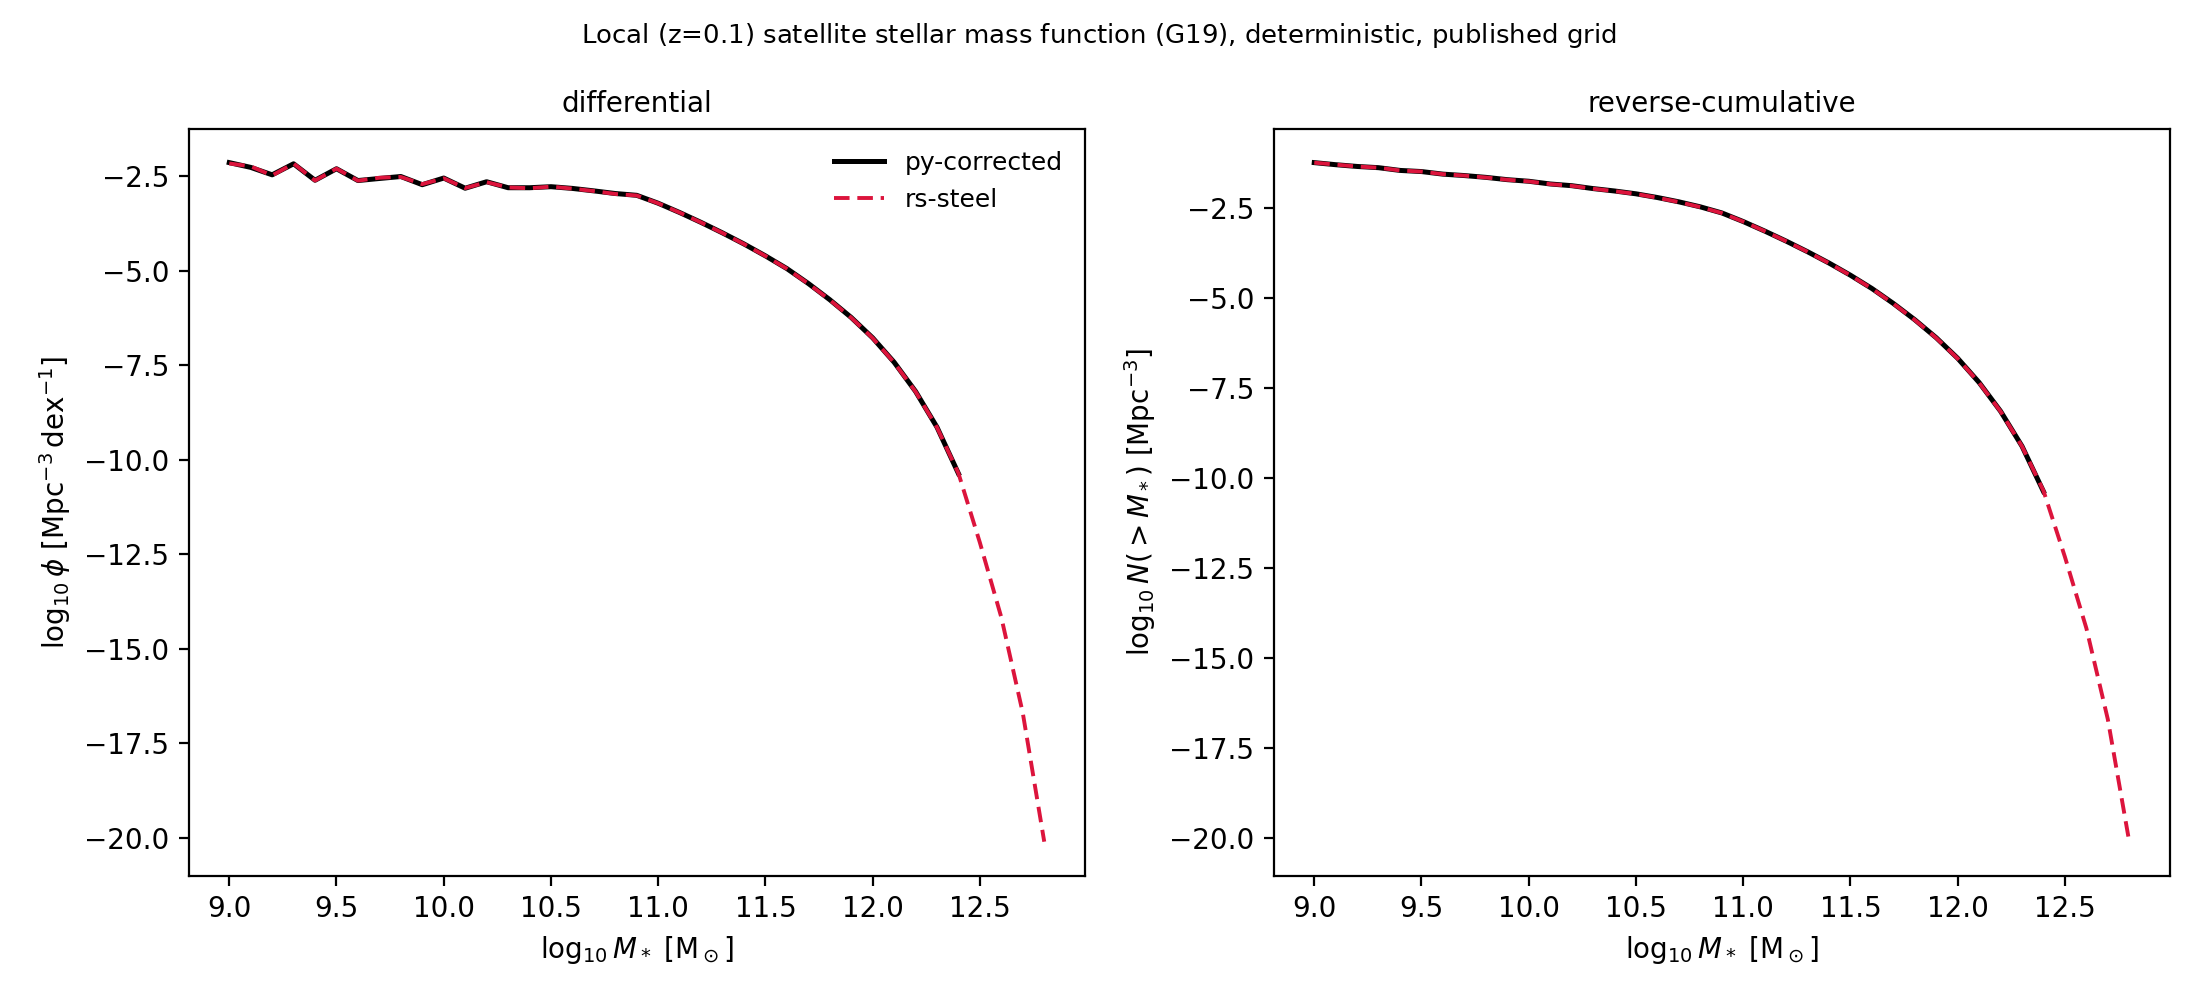
\includegraphics[width=\columnwidth]{figures/Paper1_SatelliteSMF.png}
\caption{Local ($z\sim0.1$) satellite stellar mass function, deterministic
mode, published grid: differential (left) and reverse-cumulative (right).
Solid: \texttt{py-corrected}. Dashed: \texttt{rs-steel}. Not keyed to a
specific numbered figure in Paper~1 -- see the main text.}
\label{fig:smf}
\end{figure}

\begin{figure}
\centering
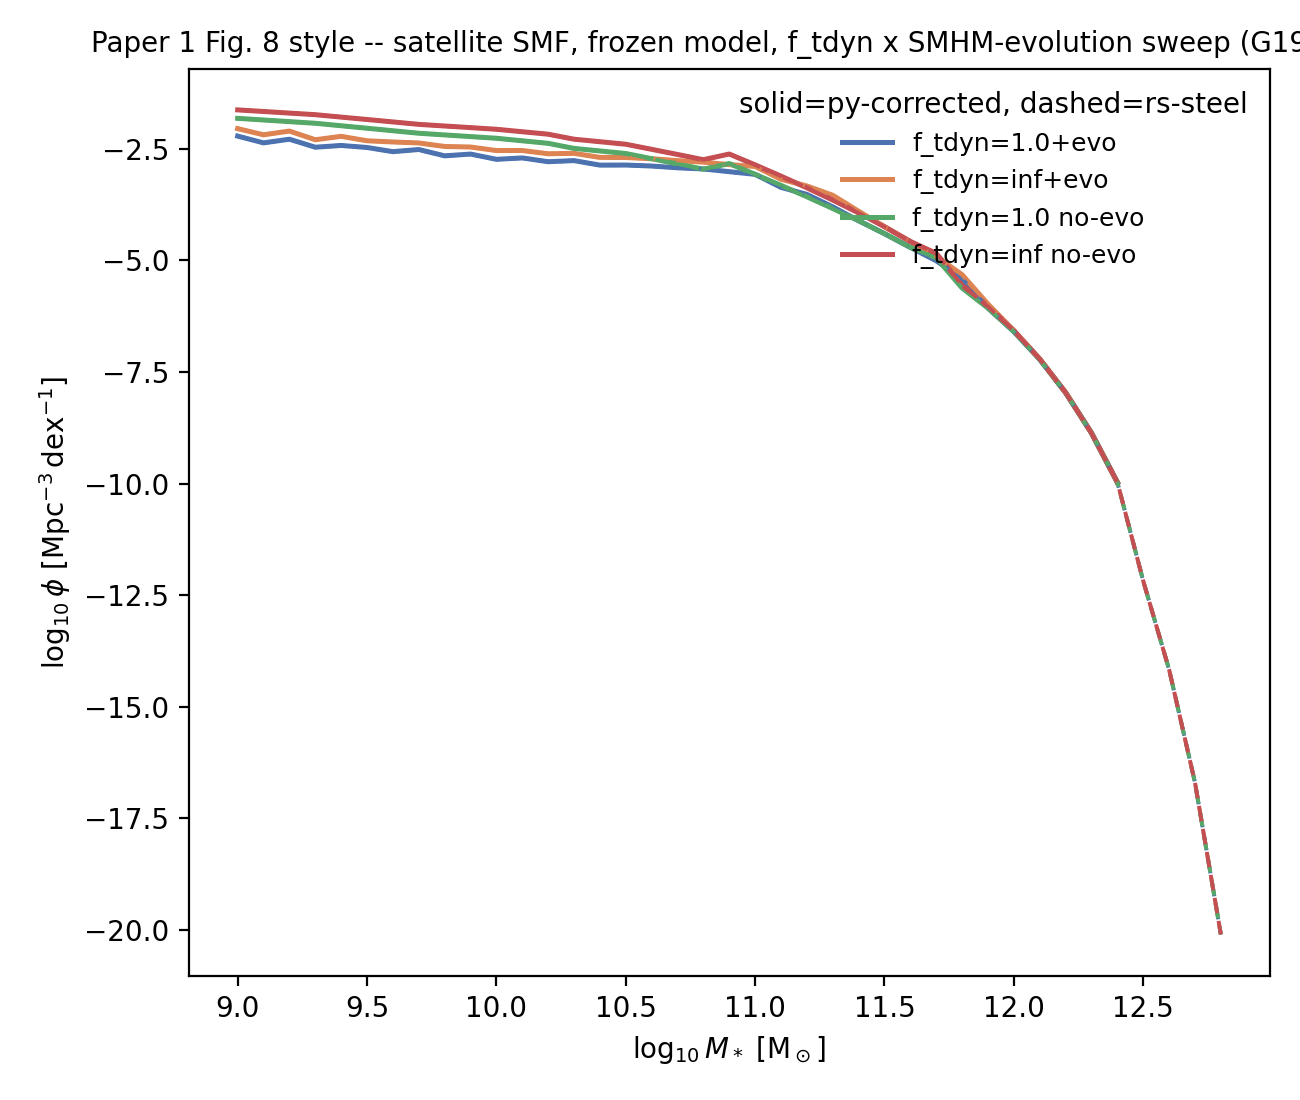
\includegraphics[width=\columnwidth]{figures/Paper1_Fig8_FrozenSweep.png}
\caption{Frozen-model satellite stellar mass function under the
$f_{\rm tdyn}\times$SMHM-evolution sweep that Paper~1 \S4.1 actually
uses (not a stellar-population comparison, which is a different figure
in the same paper). Four lines, two implementations.}
\label{fig:frozen}
\end{figure}

\begin{figure}
\centering
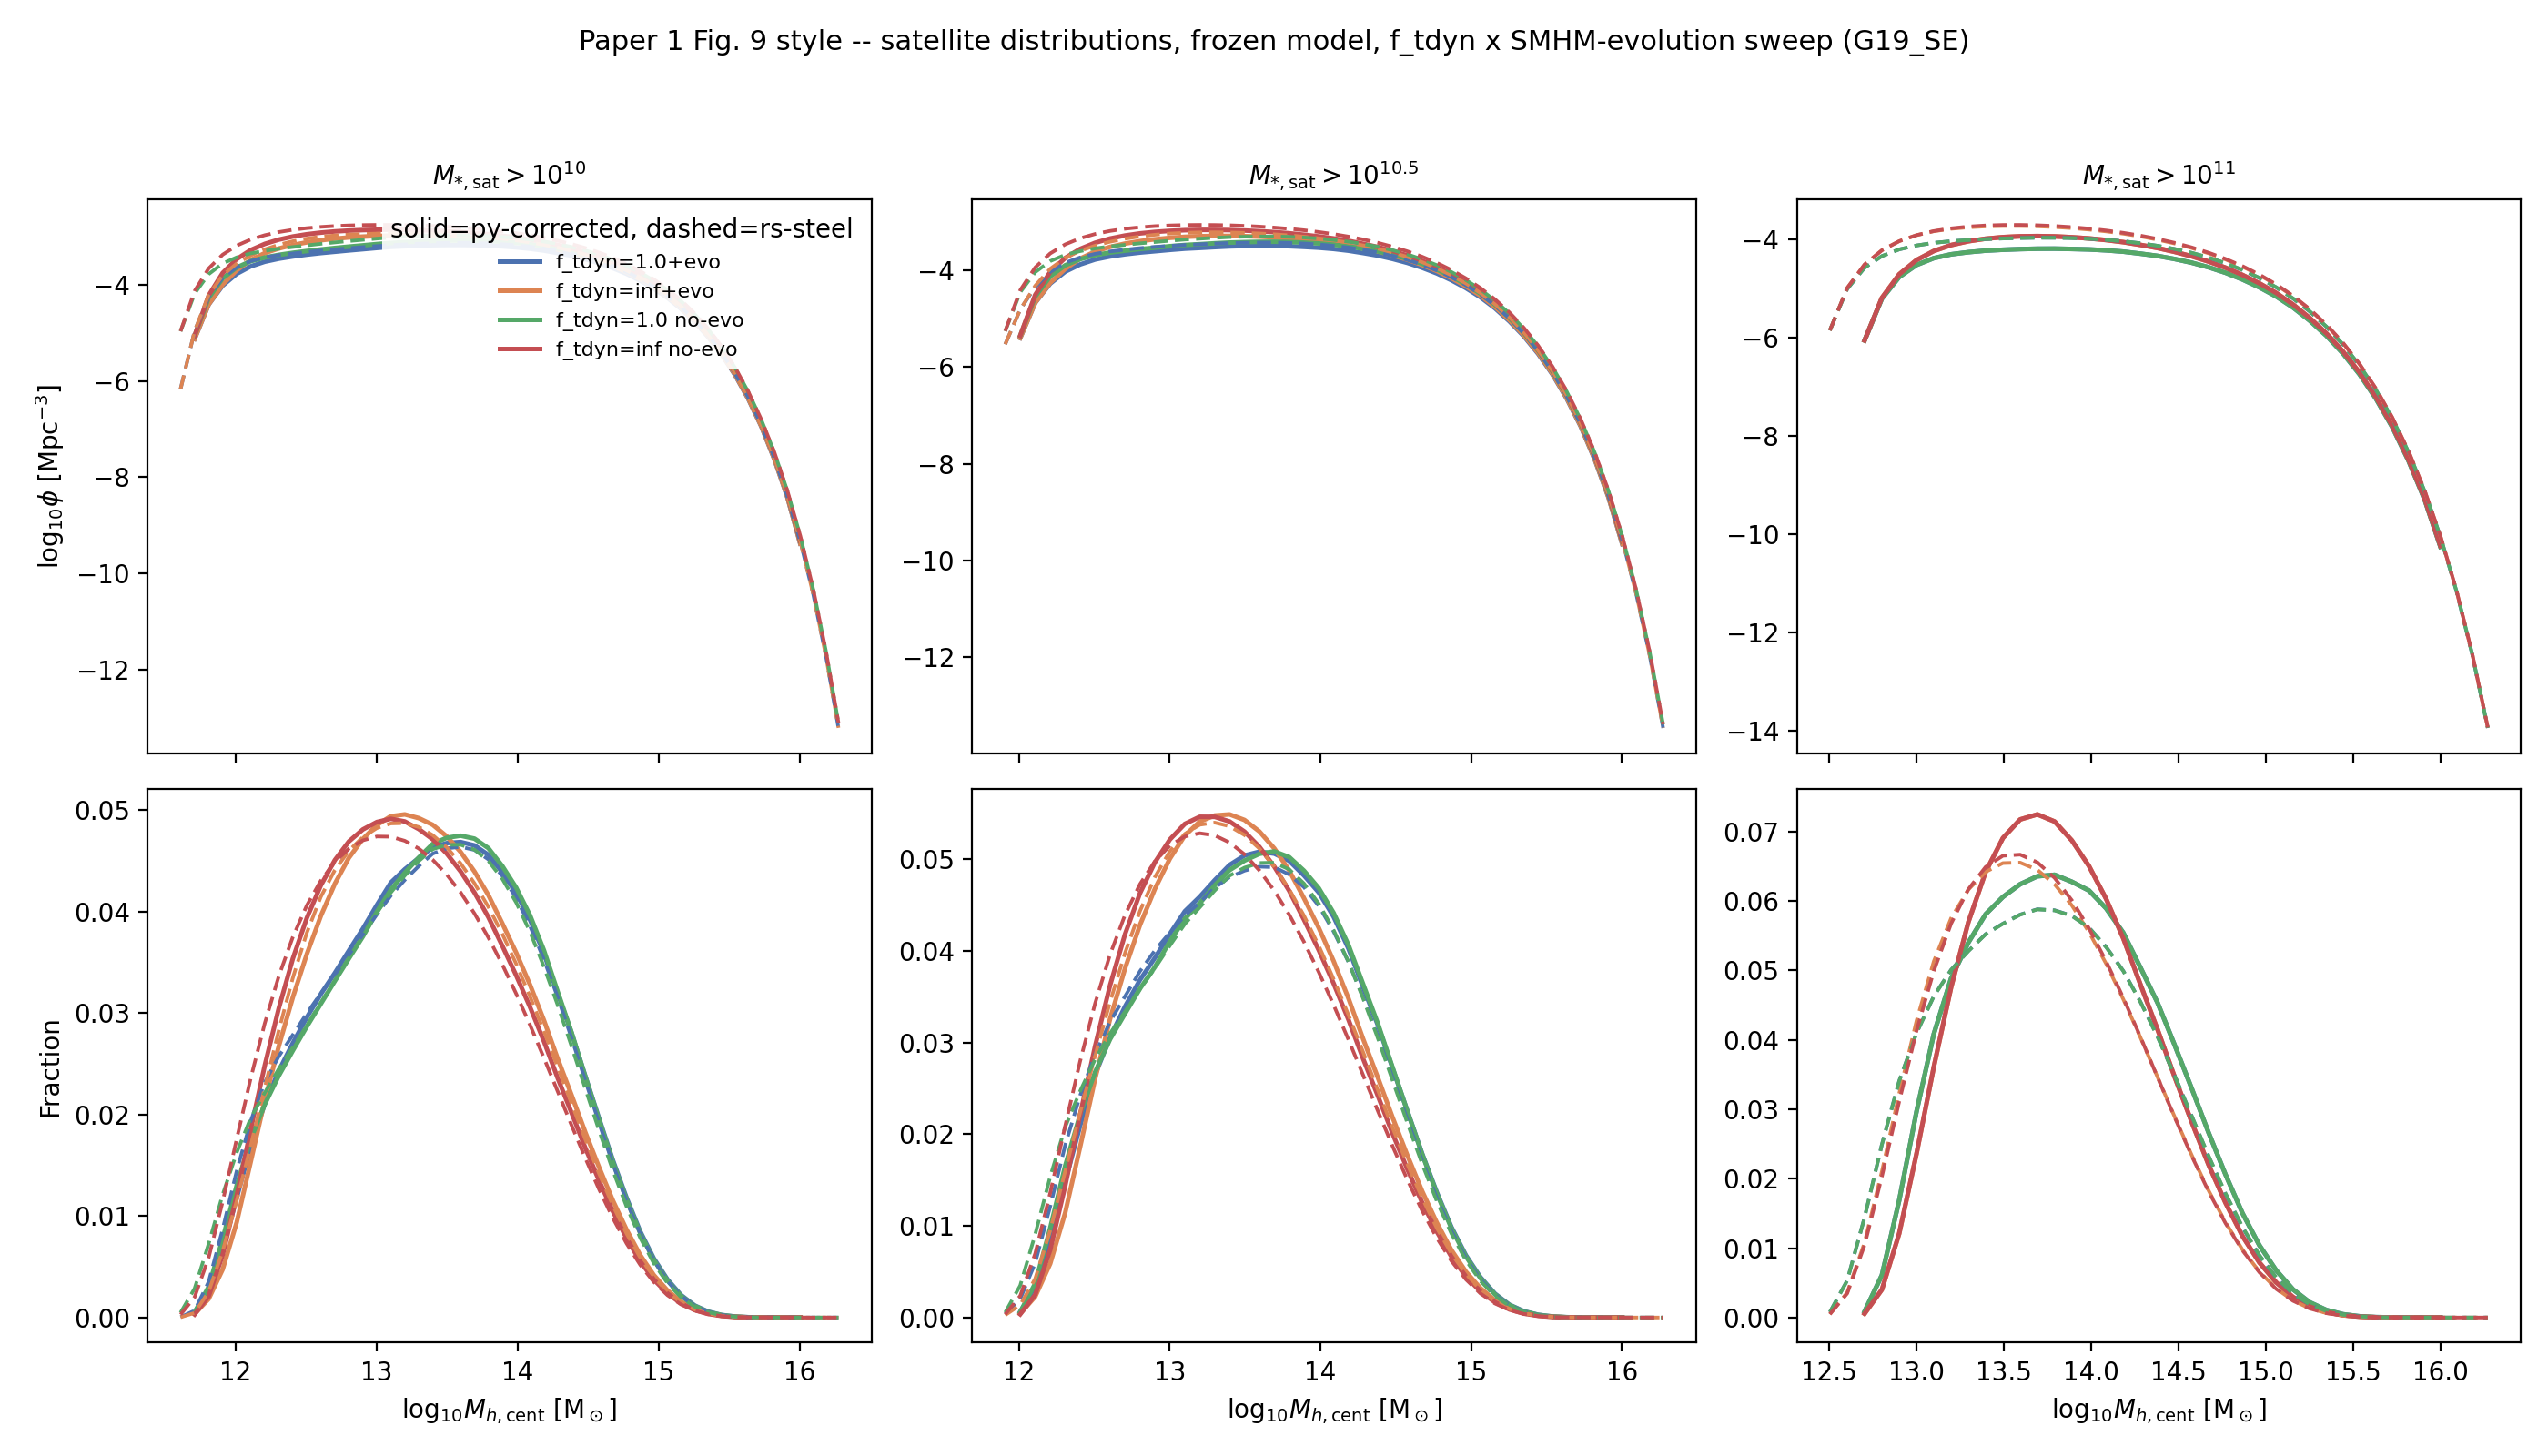
\includegraphics[width=\columnwidth]{figures/Paper1_Fig9_FrozenSweep_Grid.png}
\caption{Satellite number density (top row) and fractional distribution
(bottom row, eq.~16 of Paper~1) vs.\ parent halo mass under the same
frozen-model $f_{\rm tdyn}\times$SMHM-evolution sweep as
Fig.~\ref{fig:frozen} (Paper~1 Fig.~9), for three increasing satellite
stellar-mass cuts (columns). Four lines, two implementations.}
\label{fig:frozengrid}
\end{figure}

\begin{figure}
\centering
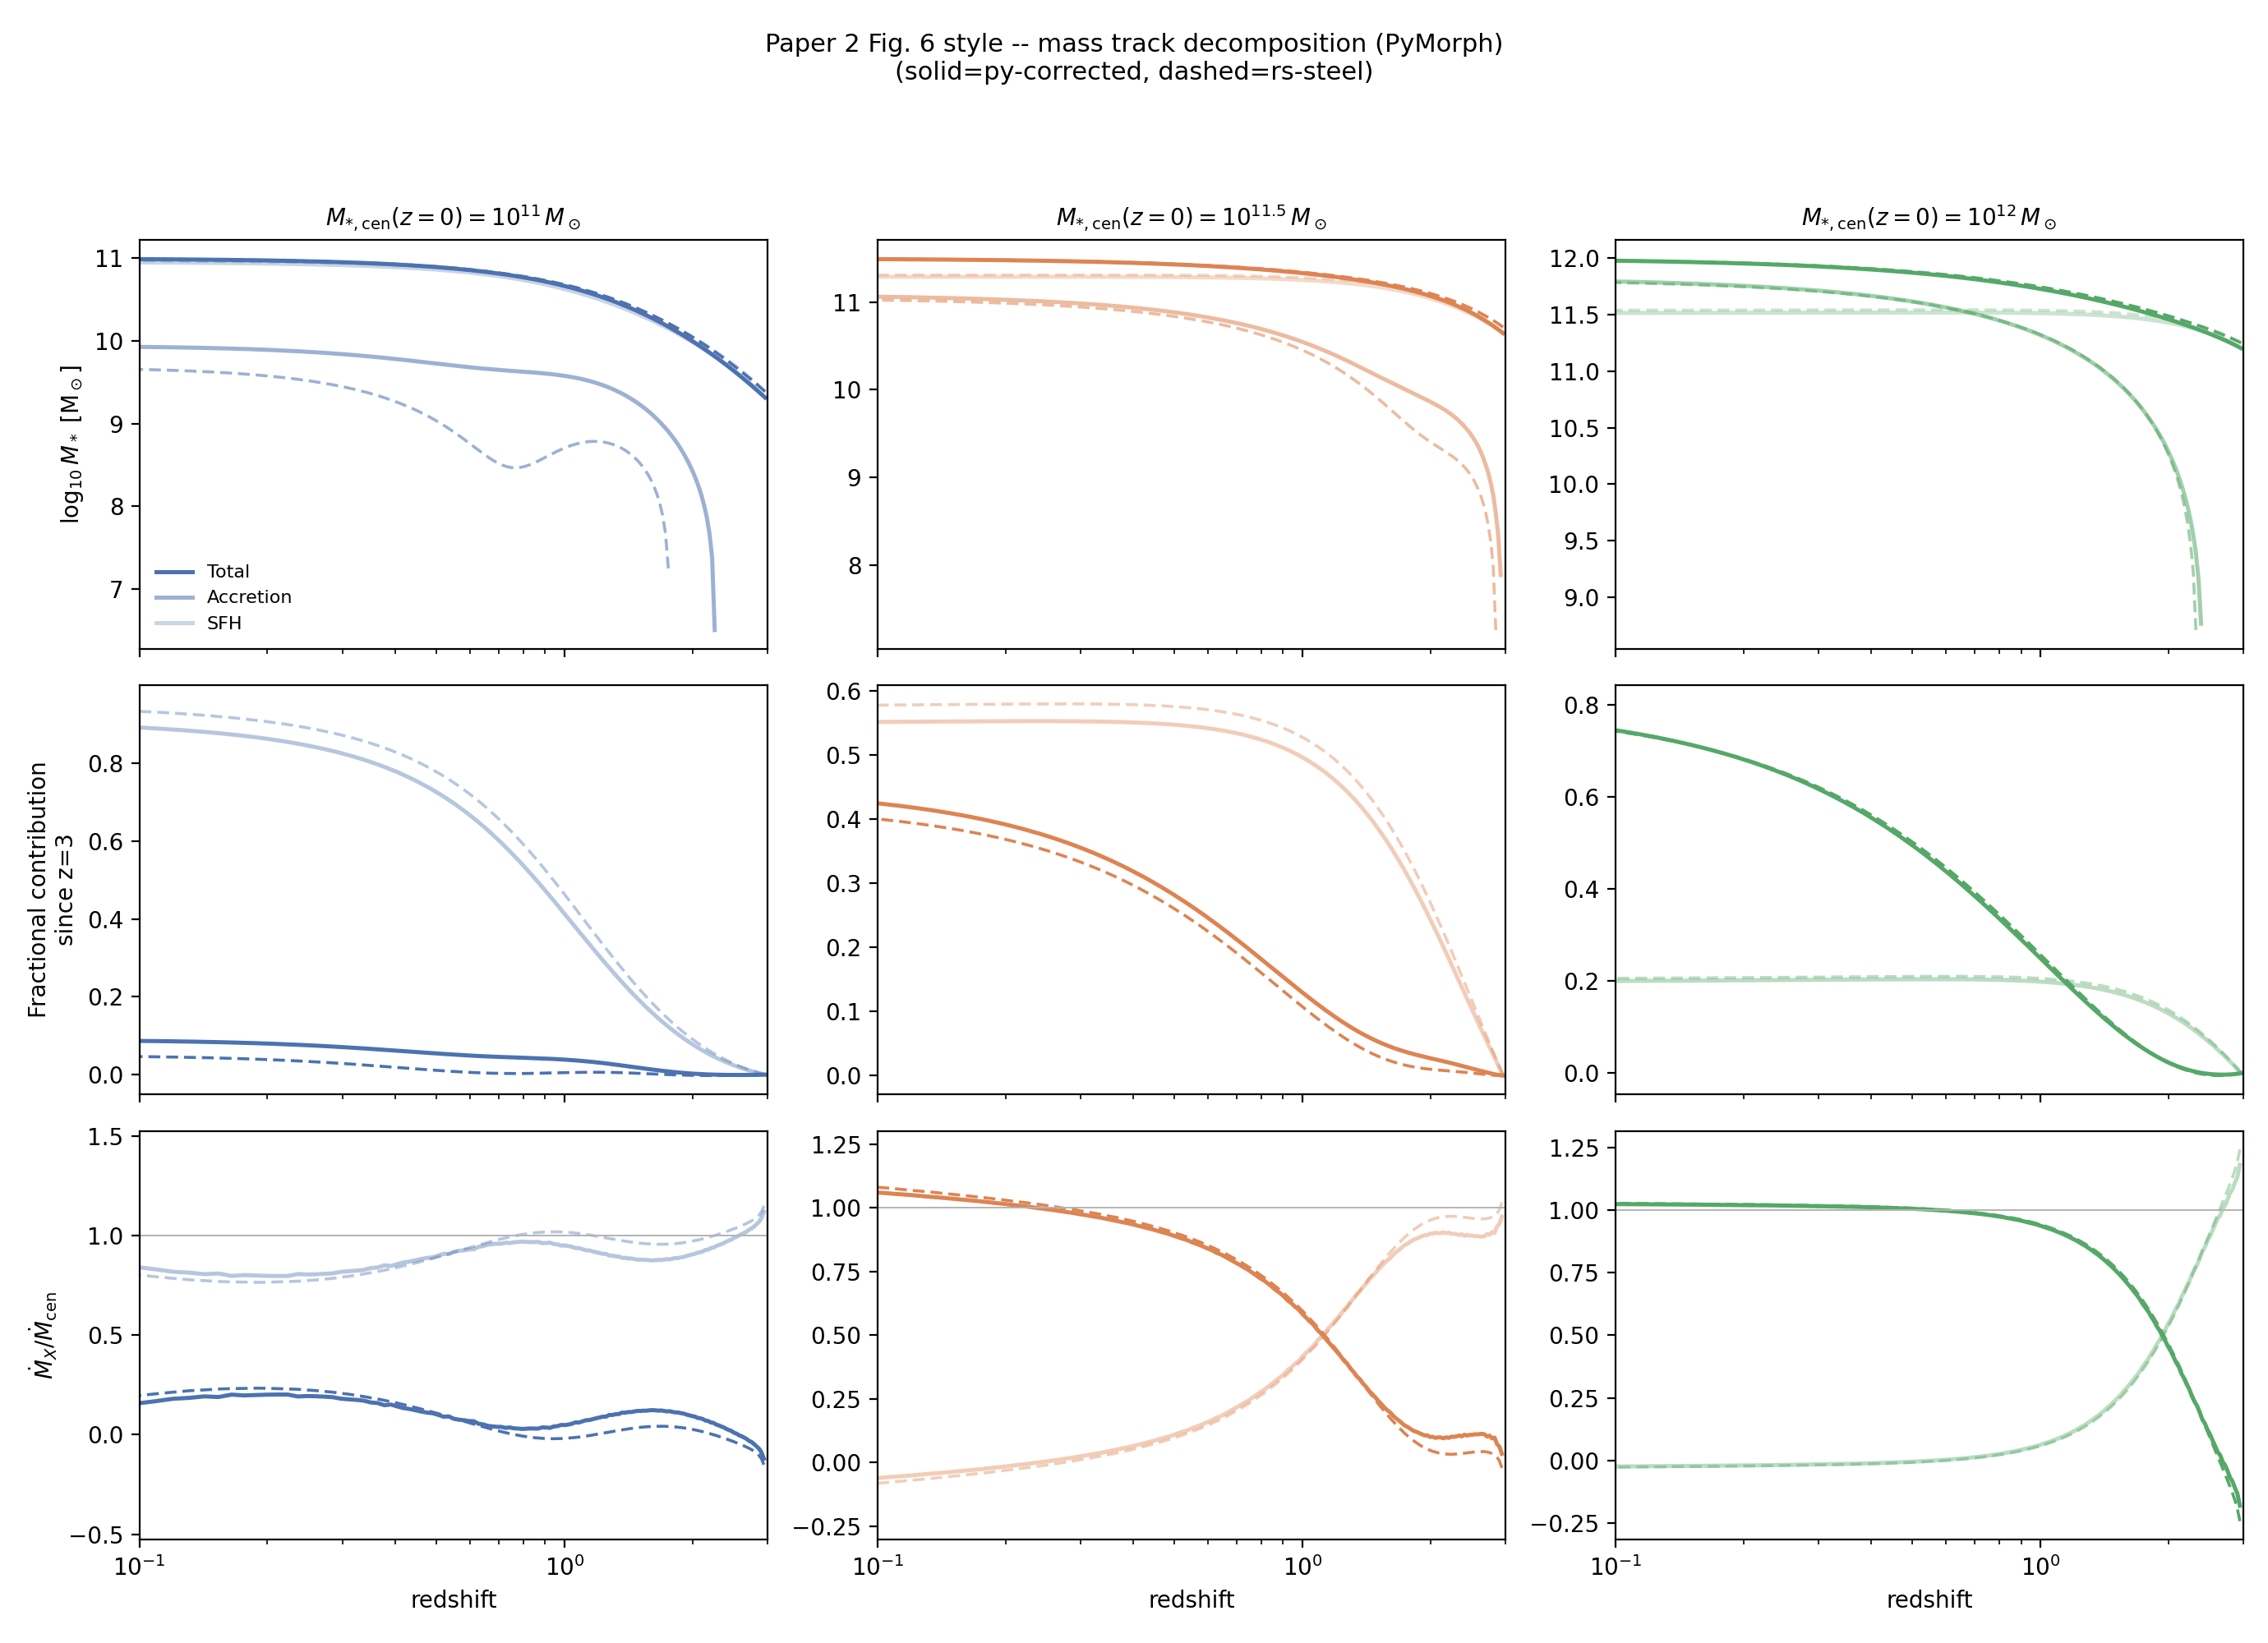
\includegraphics[width=\columnwidth]{figures/Paper2_Fig6_MassTrackDecomposition.png}
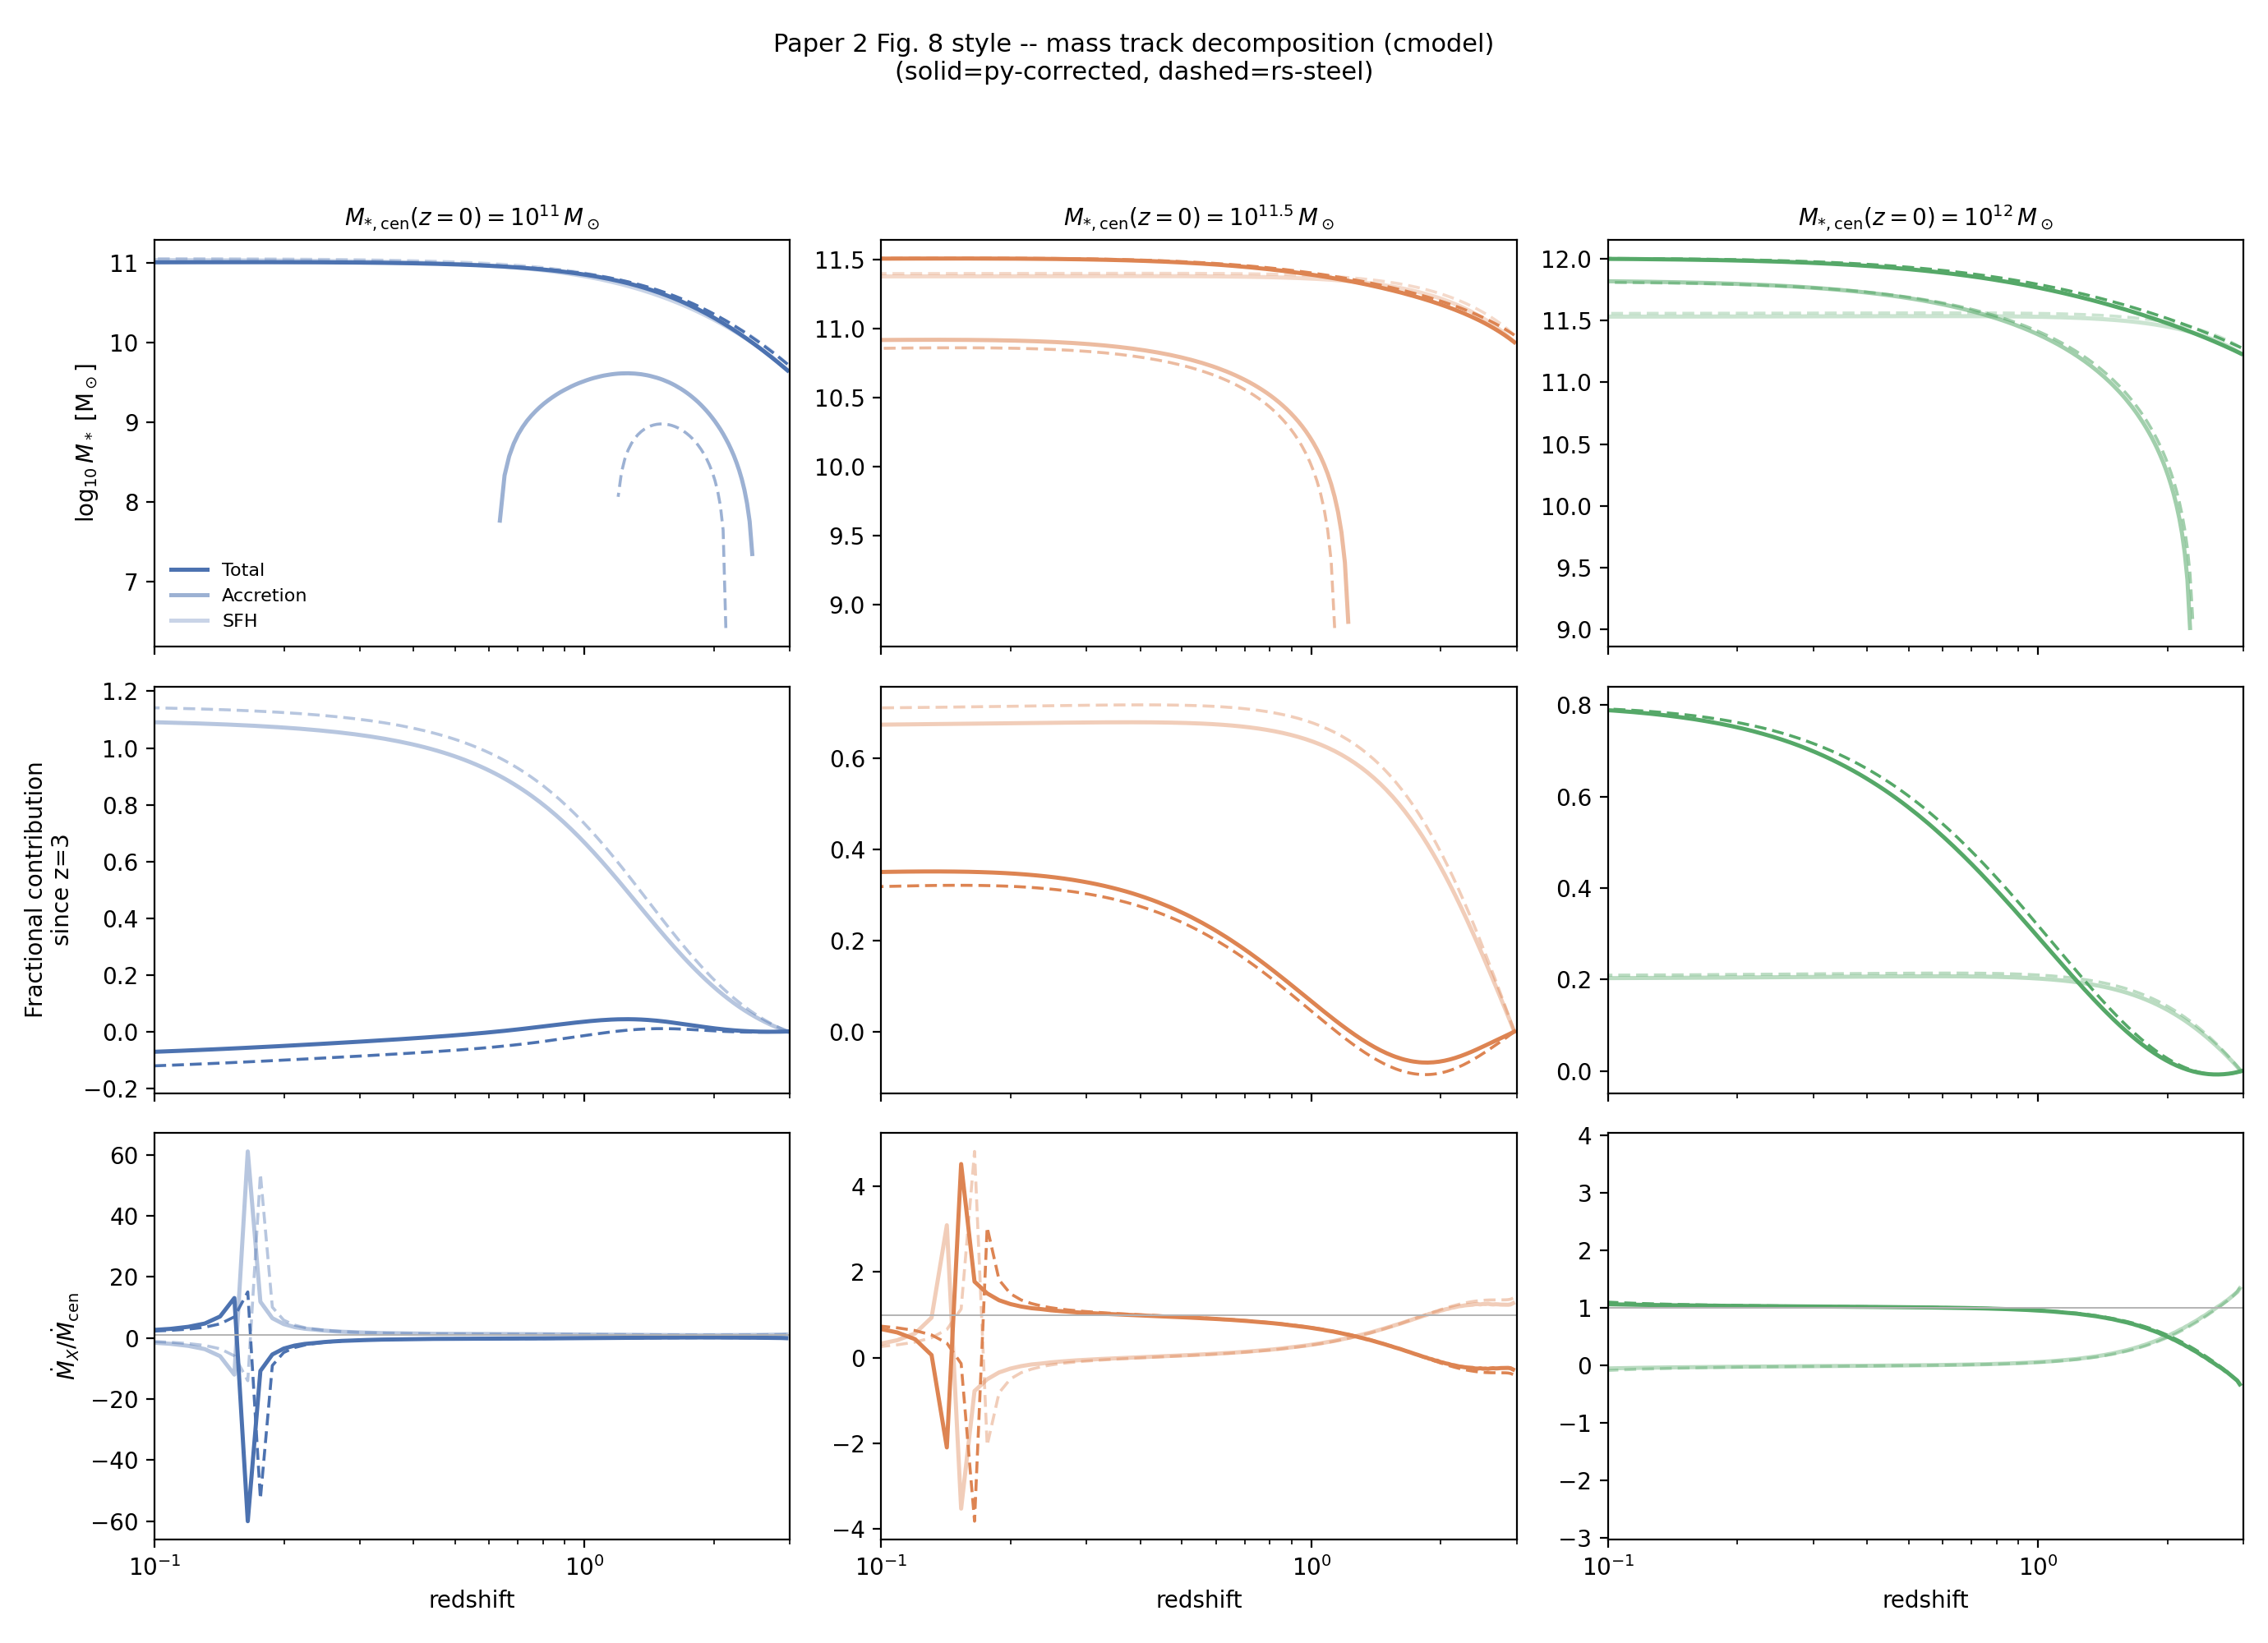
\includegraphics[width=\columnwidth]{figures/Paper2_Fig8_MassTrackDecomposition.png}
\caption{Central mass-track decomposition for the PyMorph (top) and
cmodel (bottom) stellar-mass calibrations, three target $z=0$ masses.
Top row of each panel: total, accretion, and in-situ star-formation
mass vs.\ redshift. Middle: fractional contribution to growth since
$z=3$. Bottom: instantaneous accretion-to-total growth-rate ratio. The
cmodel panel's $M_*=10^{11}\,M_\odot$ column shows the growth history
becoming internally non-physical, as the published paper itself reports
for this calibration.}
\label{fig:tracks}
\end{figure}

\begin{figure}
\centering

\includegraphics[width=\columnwidth]{figures/Paper2_Fig9_sSFR.png}
\caption{Satellite specific star-formation rate distribution in
Paper~2's three stellar-mass ranges ($10<\log M_{*,\rm sat}<10.5$,
$10.5$--$11.3$, $11.3$--$12.5$), stochastic mode, 8-seed ensemble mean
(Paper~2 Fig.~9, satellite side only -- the published figure's
central-galaxy overlay needs the dynamical-quenching post-processing
this comparison does not run). Solid: \texttt{py-corrected}. Dashed:
\texttt{rs-steel}. The quenched and star-forming peaks only separate
with scatter enabled; the highest-mass panel is thin because an
eight-seed ensemble is only tractable on a coarser grid than the full
published one (\S\ref{sec:method}).}
\label{fig:ssfr}
\end{figure}

\begin{figure}
\centering
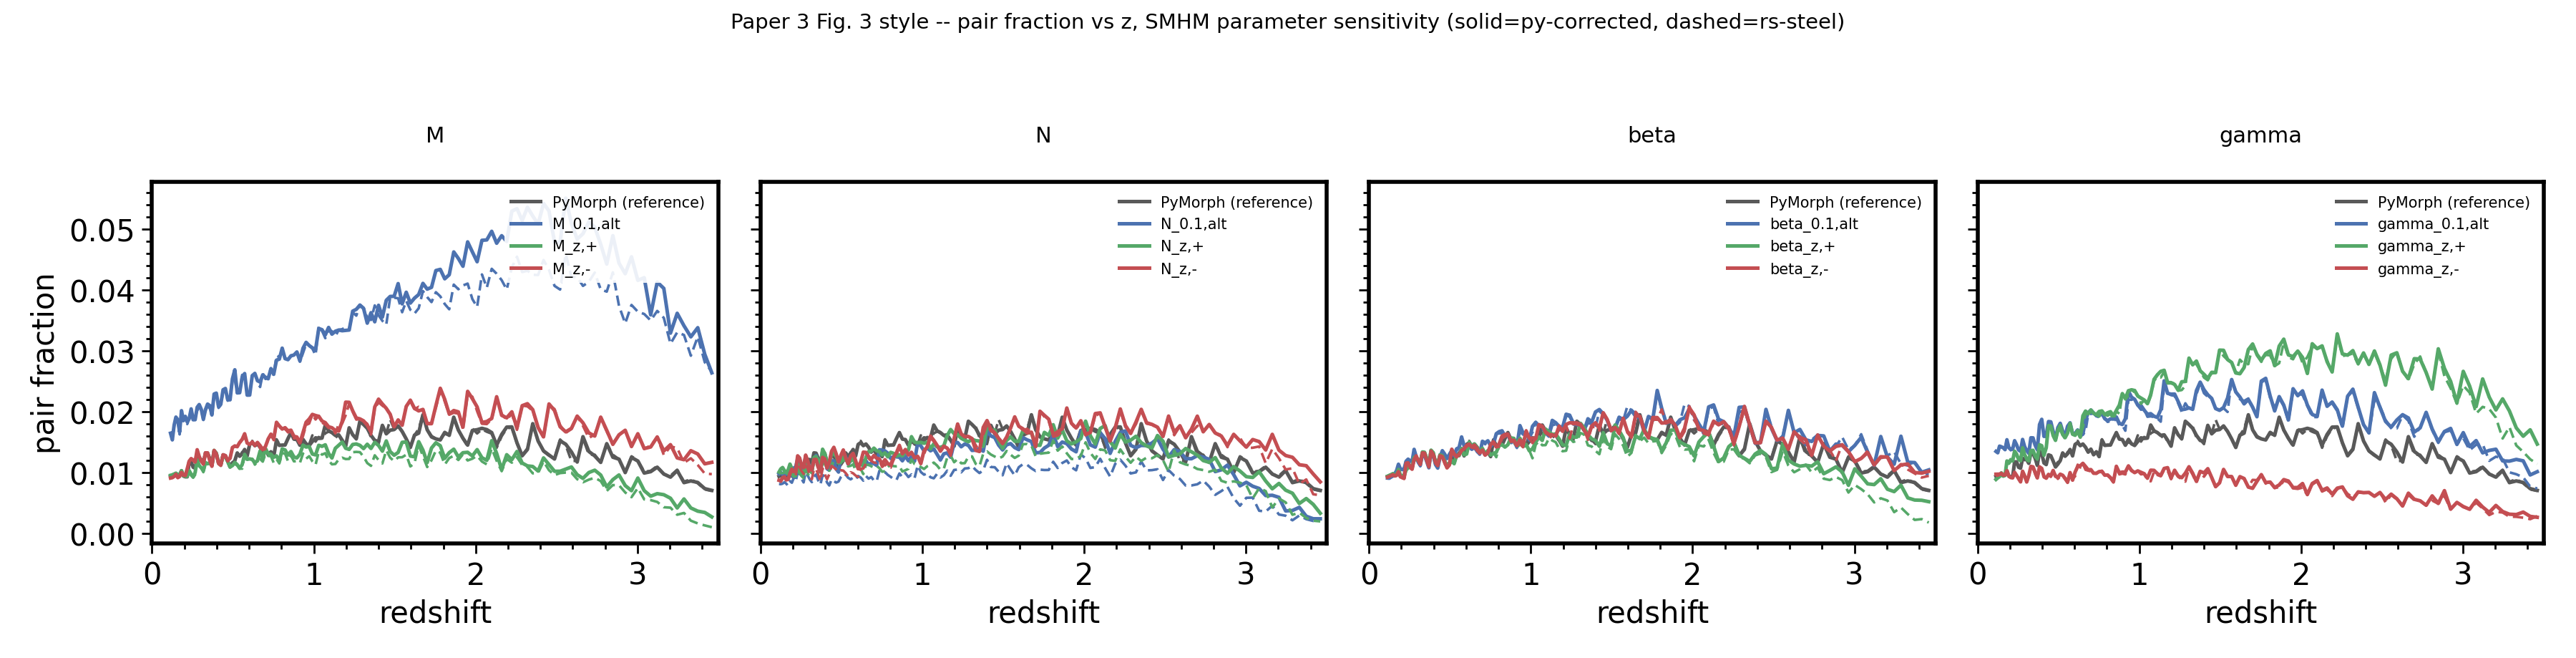
\includegraphics[width=\columnwidth]{figures/Paper3_Fig3_PairFractionSensitivity.png}
\caption{Galaxy pair fraction vs.\ redshift under thirteen
single-coefficient perturbations of the Moster-form SMHM relation
(four panels, left to right: knee mass, normalisation, low- and
high-mass slope, matching Paper~3's own Table~2), each
against a PyMorph reference. Solid: \texttt{py-corrected}. Dashed:
\texttt{rs-steel}. The high-mass slope ($\gamma$) and knee-mass ($M$)
panels show the strongest sensitivity, consistent with the published
paper's central claim that the high-mass end of the SMHM relation is the
dominant systematic in pair-fraction inference.}
\label{fig:pairfrac}
\end{figure}

\begin{figure}
\centering
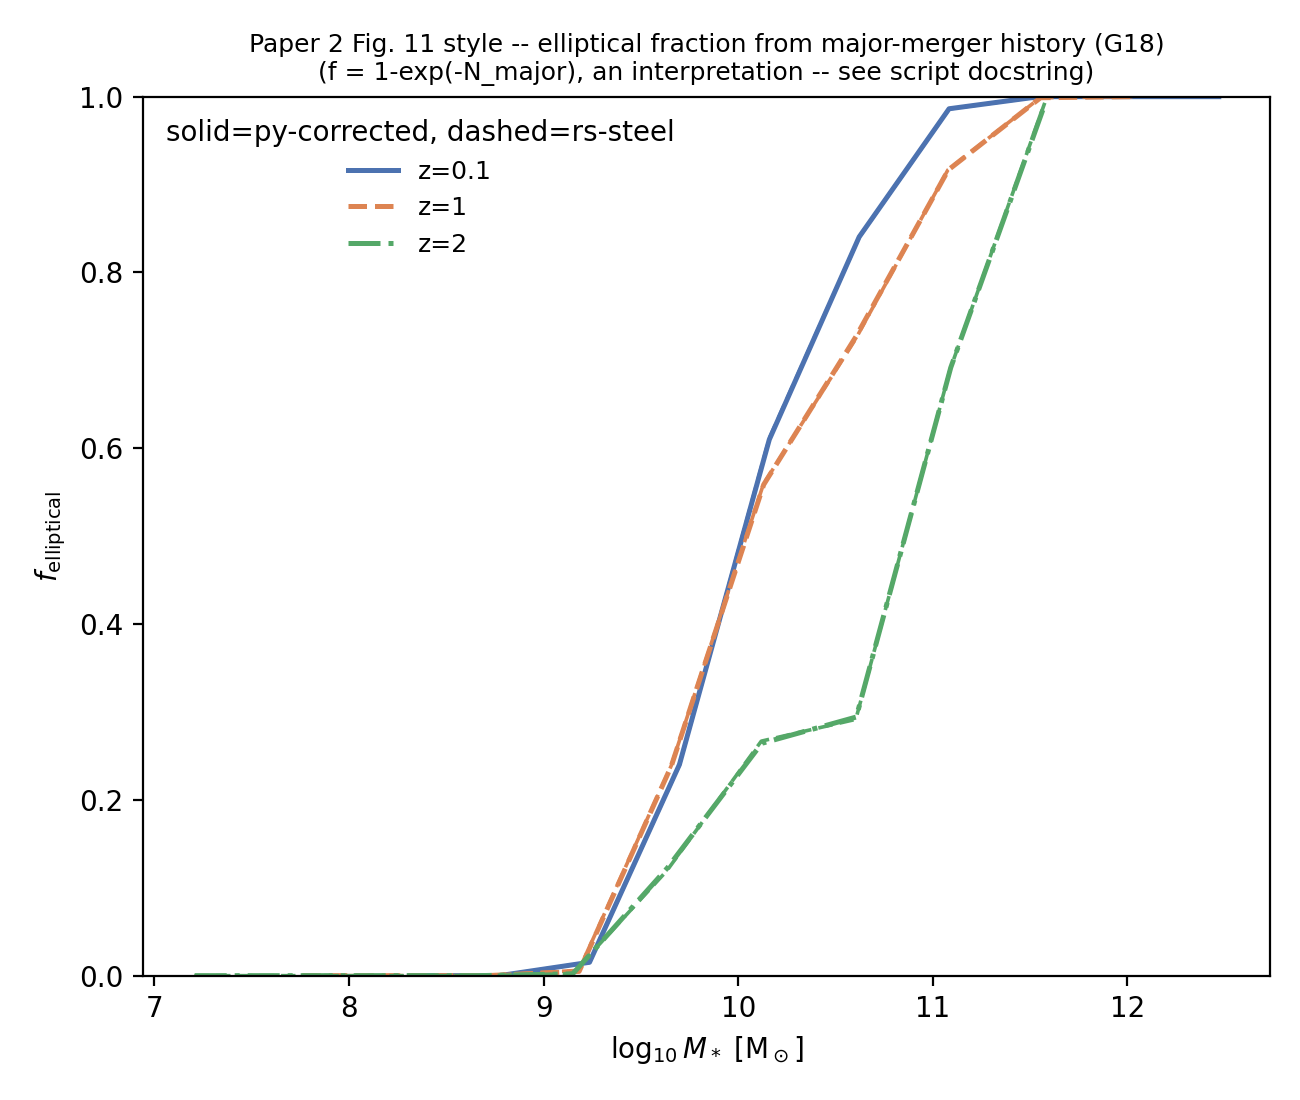
\includegraphics[width=\columnwidth]{figures/Paper2_Fig11_EllipticalFraction.png}
\caption{Elliptical fraction vs.\ stellar mass at three redshifts,
derived from each central mass track's major-merger ($\mu>0.25$)
accretion history via $f_{\rm elliptical}=1-\exp(-N_{\rm major})$.
Solid: \texttt{py-corrected}. Dashed: \texttt{rs-steel}. Qualitatively
correct shape and redshift ordering; the exact turnover mass is not
verified against the published curve, since the paper does not state
its count-to-fraction conversion.}
\label{fig:morph}
\end{figure}

\section{Discussion}
\label{sec:discuss}

The reproducibility failure in \S\ref{sec:repro} is not particular to
this code; it is what happens to any unmaintained scientific codebase
after enough major-version churn in its dependencies, and semi-empirical
models with a handful of users and no packaging discipline are
particularly exposed. What is more specific to this exercise is
\S\ref{sec:bugs}: every defect we found with a measurable effect on a
published figure was found either by reading the original code closely
enough to re-implement it independently, or by trying to reproduce that
figure and discovering the two implementations disagreed. The most
consequential of them -- the one-timestep-short evolution window and the
star-formation-history unit mismatch -- are exactly the kind of silent,
no-exception, no-warning failures that a single-language,
single-implementation test suite built from inside the same codebase is
structurally poorly positioned to catch, because the tests and the code
share the same blind spot. A from-scratch reimplementation in a
different language, with a different numerical stack and a stricter type
system, forces every implicit assumption in the original to be stated
explicitly somewhere, and the three-way deterministic/stochastic split
(\S\ref{sec:method}) lets the resulting disagreements be attributed
cleanly to either the port or the original, rather than pooled into one
number that means neither.

We do not claim this as a substitute for conventional unit testing --
several of the defects in the full list were unreachable code paths with
no effect on any output, which a targeted test would have caught more
cheaply -- but for the specific failure mode of a code path that runs,
returns a plausible-looking array, and is wrong, an independent
reimplementation checked figure-by-figure against the published results
is, in our experience building this one, a more effective net than
either code review or unit testing applied after the fact.

\section{Conclusions}

We have described a dependency-injected Rust reimplementation of the
STEEL semi-empirical galaxy model and validated it against both the
originally published code and a defect-corrected version of it, on every
headline results figure across the three papers STEEL underlies. The
port agrees with a corrected Python implementation to better than
$0.5\%$ on every integrated quantity compared in deterministic mode, runs
$4.5\times$ faster on the published parameter grid, and its construction
surfaced defects -- most consequentially a one-timestep-short satellite
evolution window and a unit mismatch in the star-formation-history
accumulator -- that shift the shape of the merger accretion history and
pair-fraction outputs Papers 2 and 3 build their headline results on by
tens of per cent, though the integrated stellar mass function moves by
under one. We make the port, the corrected Python branch, and the full
defect catalogue available at \url{https://github.com/PipGrylls/STEEL}.

\section*{Data Availability}
The Rust port, the corrected Python branch, the validation harness, and
every figure and number in this letter are available at
\url{https://github.com/PipGrylls/STEEL}. No new observational data were
used.

\bibliographystyle{mnras}
\begin{thebibliography}{}
\bibitem[Boylan-Kolchin et al.(2008)]{BoylanKolchin2008} Boylan-Kolchin M., Ma C.~P., Quataert E., 2008, MNRAS, 383, 93
\bibitem[Despali et al.(2016)]{Despali2016} Despali G., Giocoli C., Angulo R.~E., Tormen G., Sheth R.~K., Moscardini L., Baso G., 2016, MNRAS, 456, 2486
\bibitem[Eisenstein \& Hu(1998)]{EisensteinHu1998} Eisenstein D.~J., Hu W., 1998, ApJ, 496, 605
\bibitem[Grylls et al.(2019)]{Grylls2019a} Grylls P.~J., Shankar F., Zanisi L., Bernardi M., 2019, MNRAS, 483, 2506
\bibitem[Grylls et al.(2020a)]{Grylls2020} Grylls P.~J., Shankar F., Leja J., Menci N., Moster B., Behroozi P., Zanisi L., 2020, MNRAS, 491, 634
\bibitem[Grylls et al.(2020b)]{Grylls2020b} Grylls P.~J., Shankar F., Conselice C., 2020, arXiv:2001.06017
\bibitem[Jiang \& van den Bosch(2016)]{JiangVandenBosch2016} Jiang F., van den Bosch F.~C., 2016, MNRAS, 458, 2848
\bibitem[McCavana et al.(2012)]{McCavana2012} McCavana M., Micic M., Lewis G.~F., Sinha M., Sharma S., Holley-Bockelmann K., 2012, MNRAS, 424, 361
\bibitem[Mundy et al.(2017)]{Mundy2017} Mundy C.~J., Conselice C.~J., Duncan K.~J., Almaini O., H\"{a}u{\ss}ler B., Hartley W.~G., 2017, MNRAS, 470, 3507
\bibitem[van den Bosch et al.(2014)]{vandenBosch2014} van den Bosch F.~C., Jiang F., Campbell D., Watson D., Padmanabhan N., 2014, MNRAS, 445, 1713
\end{thebibliography}

\bsp
\label{lastpage}
\end{document}
